\documentclass{article}
\usepackage[utf8]{inputenc}
\usepackage{ctex}
\usepackage{graphicx}   
\usepackage{float}
\usepackage{enumerate}
\usepackage{listings}
\usepackage{booktabs}
\usepackage{multirow}
\lstset{breaklines=true}
\title{这是一篇用LaTeX写的LaTeX教程}
\author{IT工匠}
\date{May 2019}

\begin{document}
\maketitle
\begin{abstract}
    很多人习惯使用word写文档,这对普通人来说足够用了,但是对于需要撰写专业文档的工程师来说不仅操作太过复杂,而且很多需求无法满足(比如对公式和代码的支持),一部分对公式要求不是很严格的工程师会选择使用markdown写文档,特点是轻量级、对代码支持好、上手难度小、满足不那么正规的文档交流,而如果需要书写更专业的文档,比如简历、论文等,就需要更正规的工具了——LaTeX,LaTeX的特点是完美支持各种公式和符号、排版简约美观,但是上手难度相比markdown略大,本文是笔者在使用LaTeX的一些总结,相信可以满足初学者的日常需求。接下来是广告时间:本文使用纯LaTeX编写,关注微信公众号\textbf{"IT工匠”},后台回复“O3”(注意是大写字母欧不是零)可获取本文LaTeX源代码(强烈建议大家研读一下本文源码,因为很多东西由于时间原因都没介绍到,比如如何插入代码、如何生成目录等,但是在本文均有使用,相信大家看一遍源码就都懂了)以及本文pdf,另外还附赠一份我个人和女朋友(代号小草莓,公众号\textbf{"烂草莓"})一直在用\textbf{LaTeX中文简历模板},转载请注明出处。
\end{abstract}
\newpage
\tableofcontents

\section{OverLeaf入门}
\subsection{OverLeaf概述}
Overleaf是一个使用LaTeX进行多人协同编辑的平台,可以免费注册和使用,不用下载LaTeX软件,是最为著名的LaTeX在线协作系统。主要特色是有LaTeX插件,编辑功能十分完善,有实时预览(即编即看,无需手动编译)的功能。科研工作者可以在各大期刊的网站上下载到其Overleaf模板,进行论文写作(不同模板的排版方式(比如“作者”和“地址”)的格式不同)。平台是纯英文的,需要使用者适应,这也是优秀的工程师应该具备的基本素养。
\subsection{OverLeaf使用}
OverLeaf的网址是:https://www.overleaf.com,进入网站后,首页如图\ref{overleaf-main-page}所示,大家可以根据自己的情况使用第三方账号进行登录。

\begin{figure}[H] 
\centering
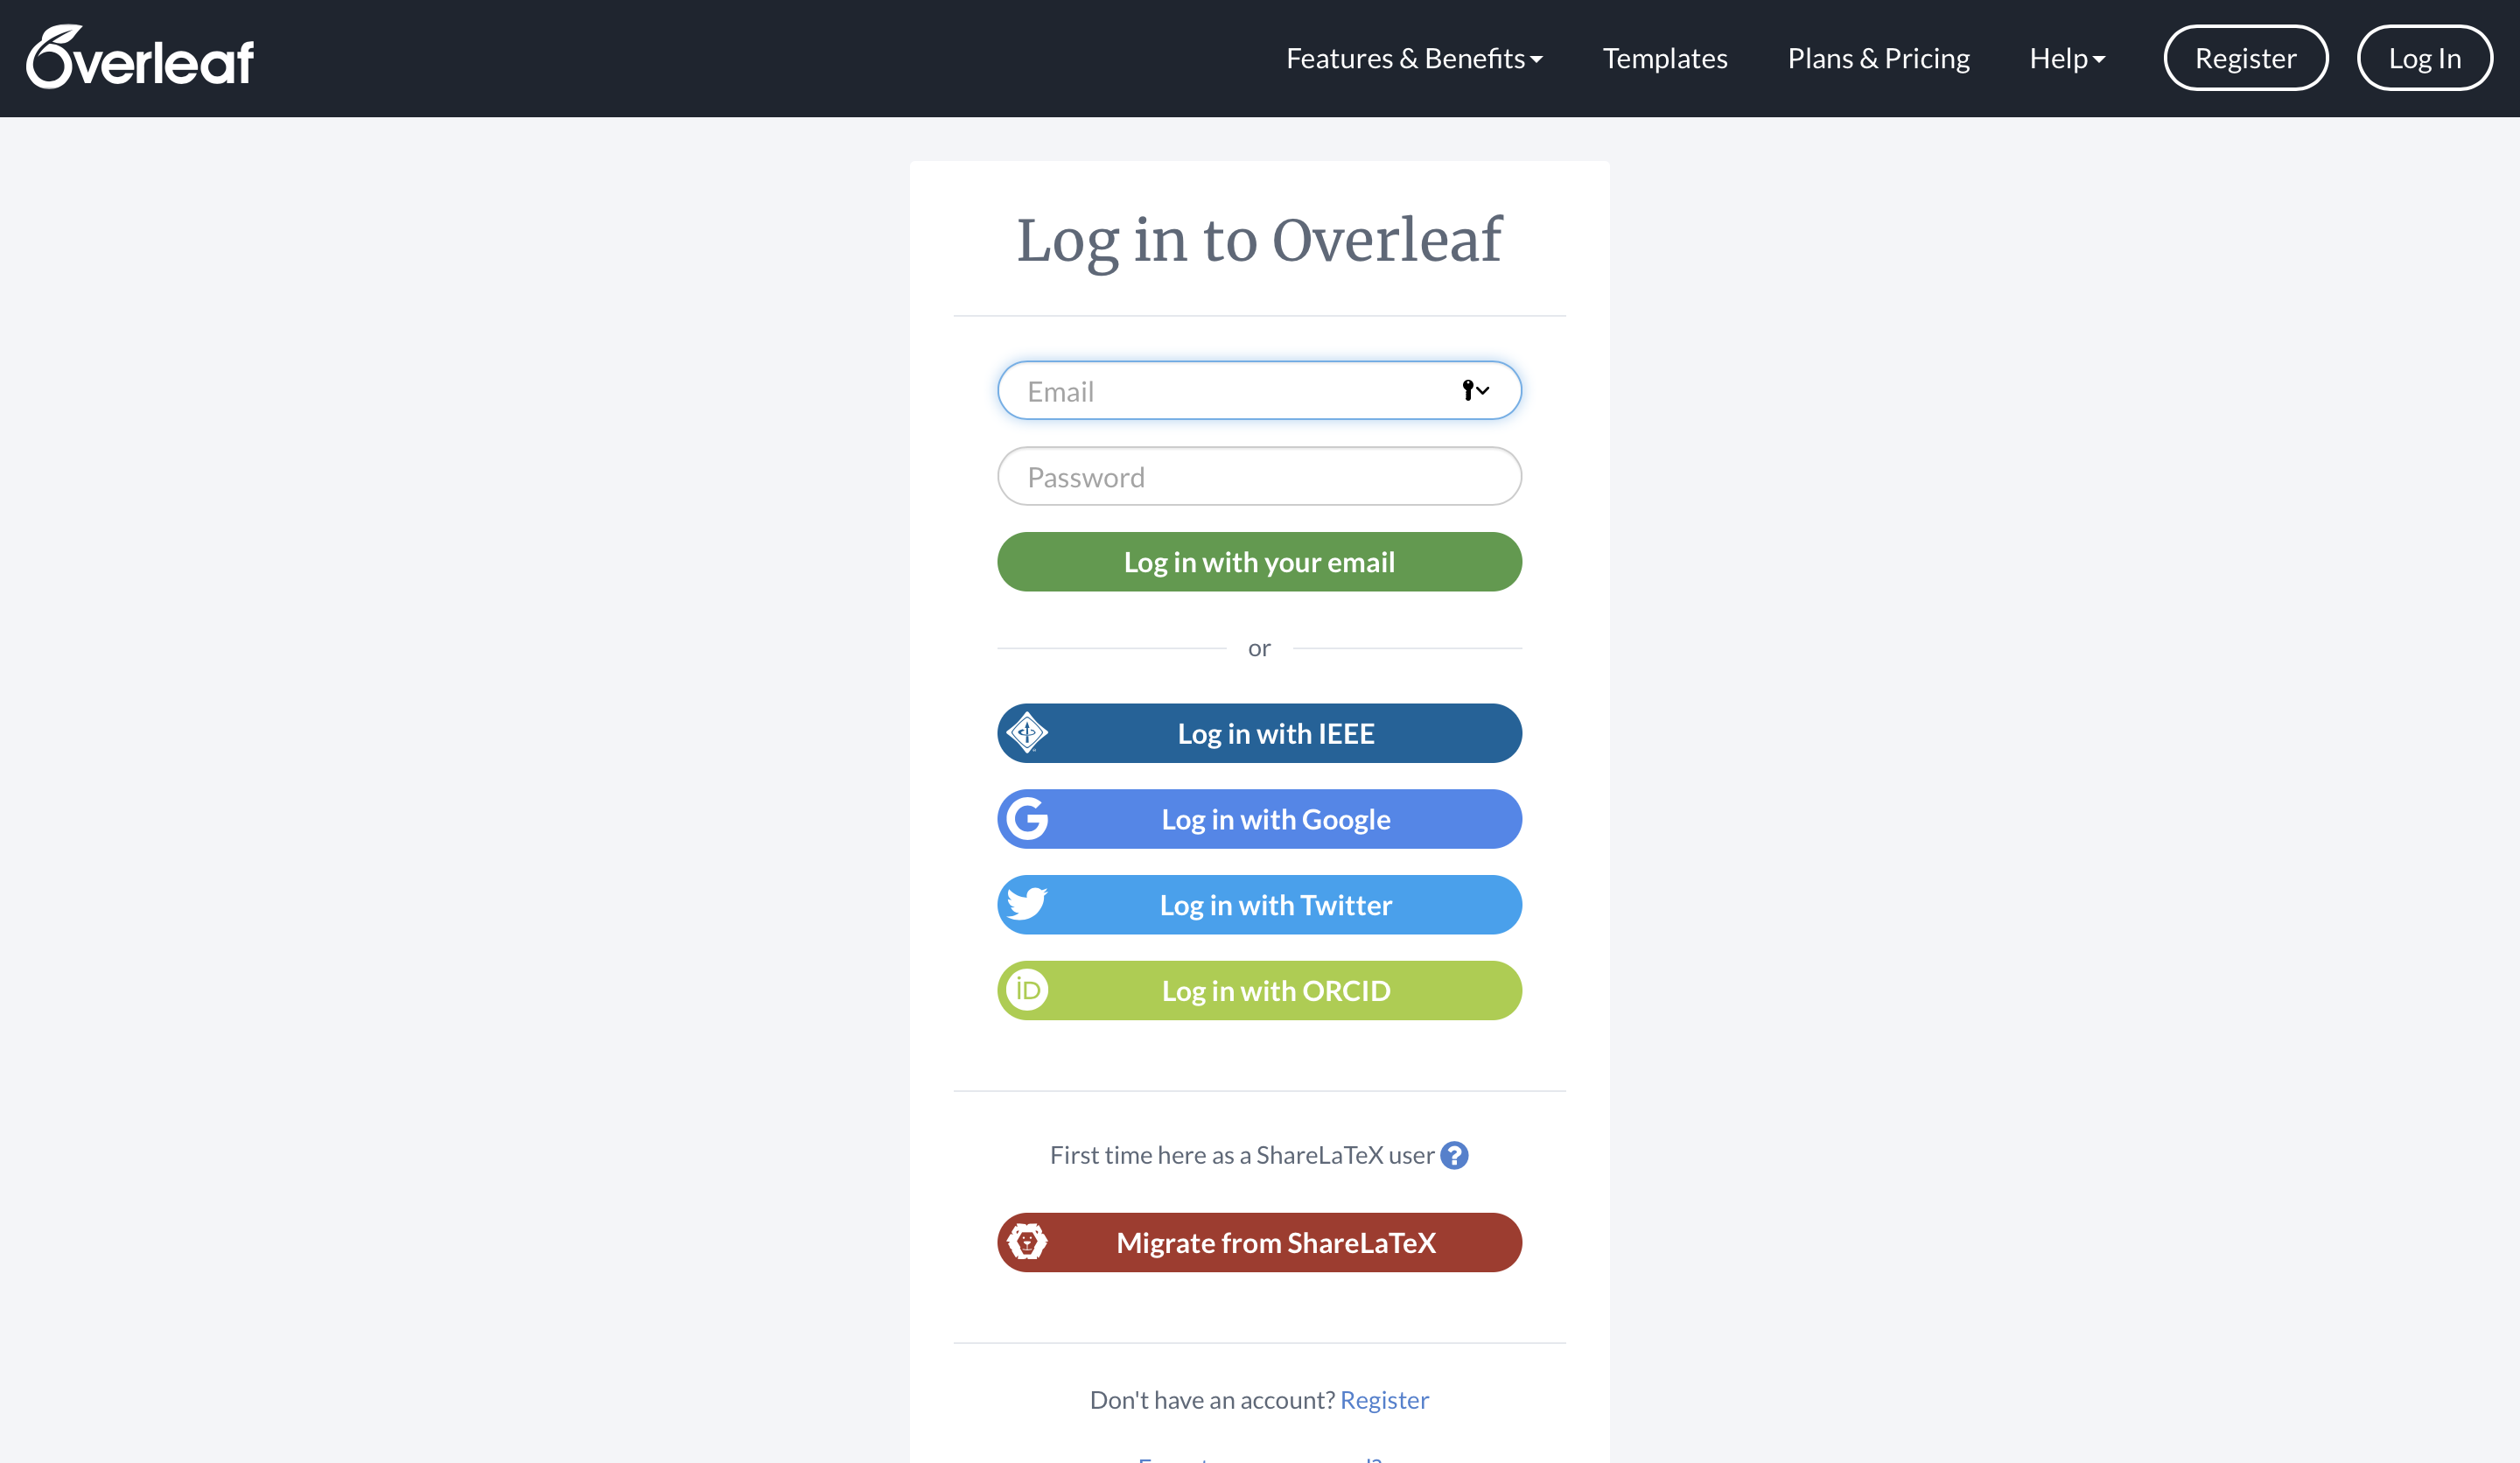
\includegraphics[width=1\textwidth]{overleaf首页.png}
\caption{OverLeaf首页}
\label{overleaf-main-page}
\end{figure}


登录成功后就可以创建项目,如图\ref{create-project-page}所示,直接选择Blank Project即可.


\begin{figure}[H]
\centering
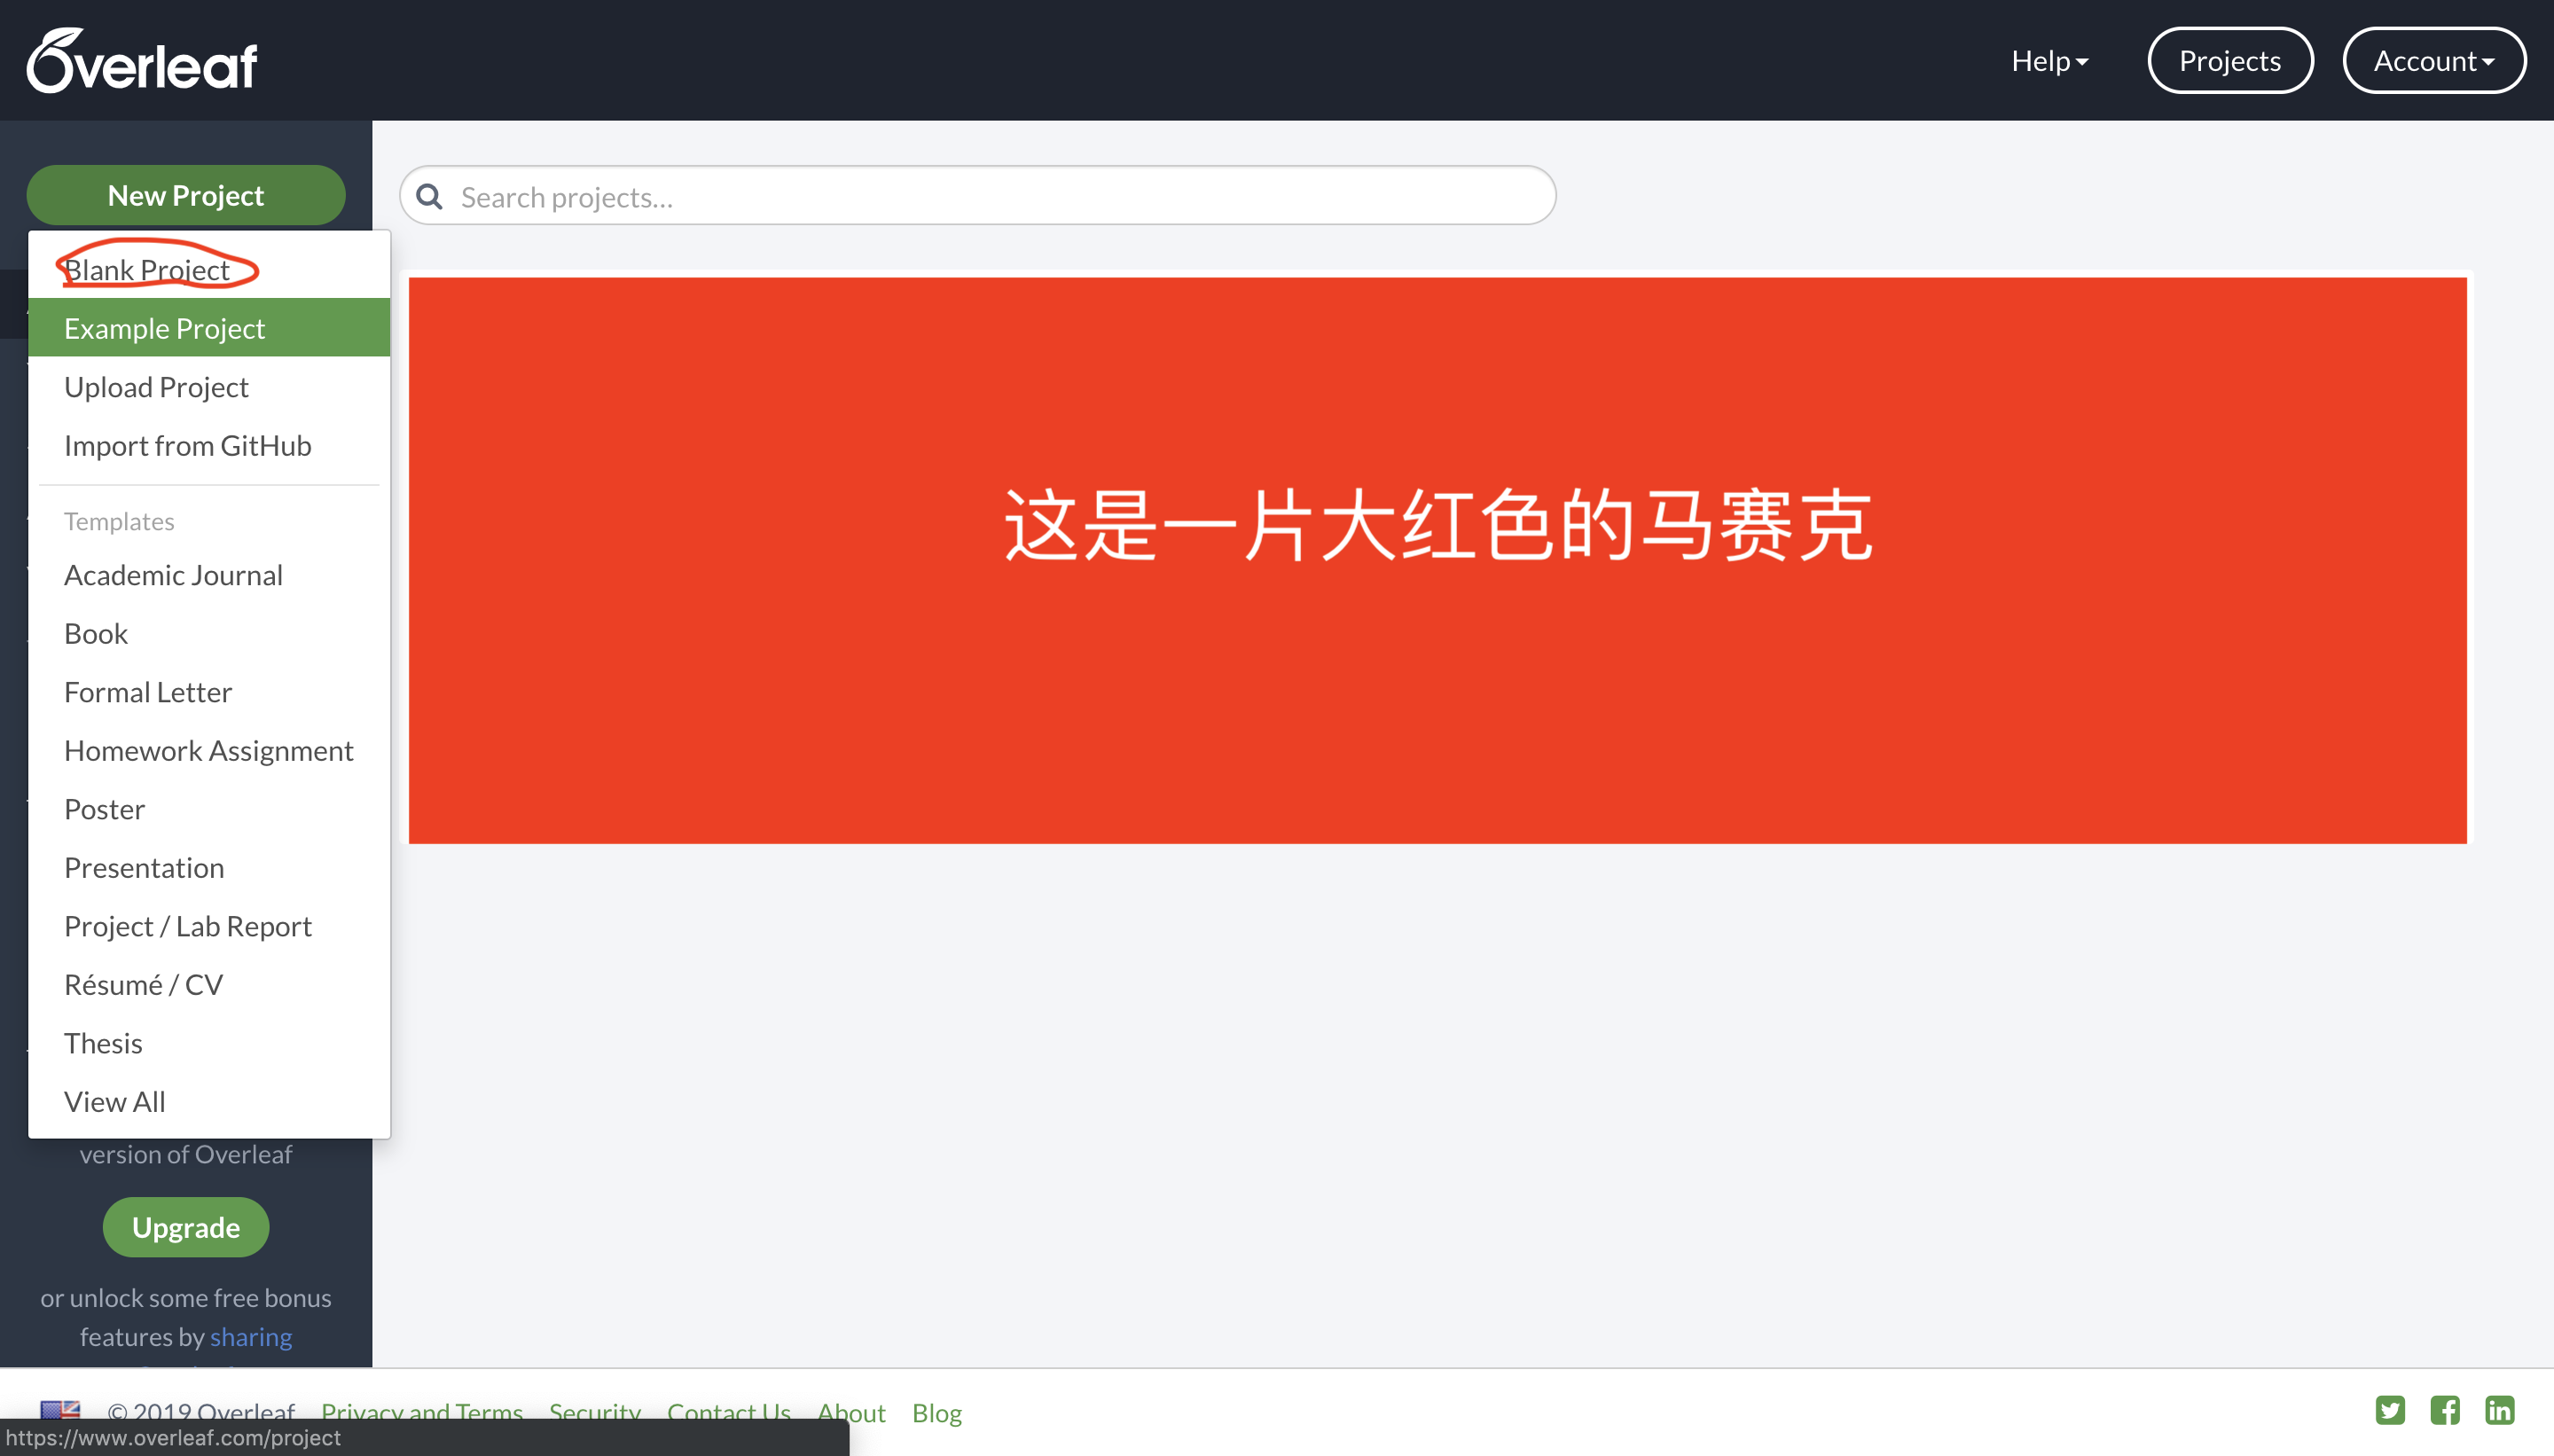
\includegraphics[width=1\textwidth]{创建项目.png}
\caption{创建项目}
\label{create-project-page}
\end{figure}
项目新建完成后初始页面如\ref{init-page}所示:

\begin{figure}[H]
\centering
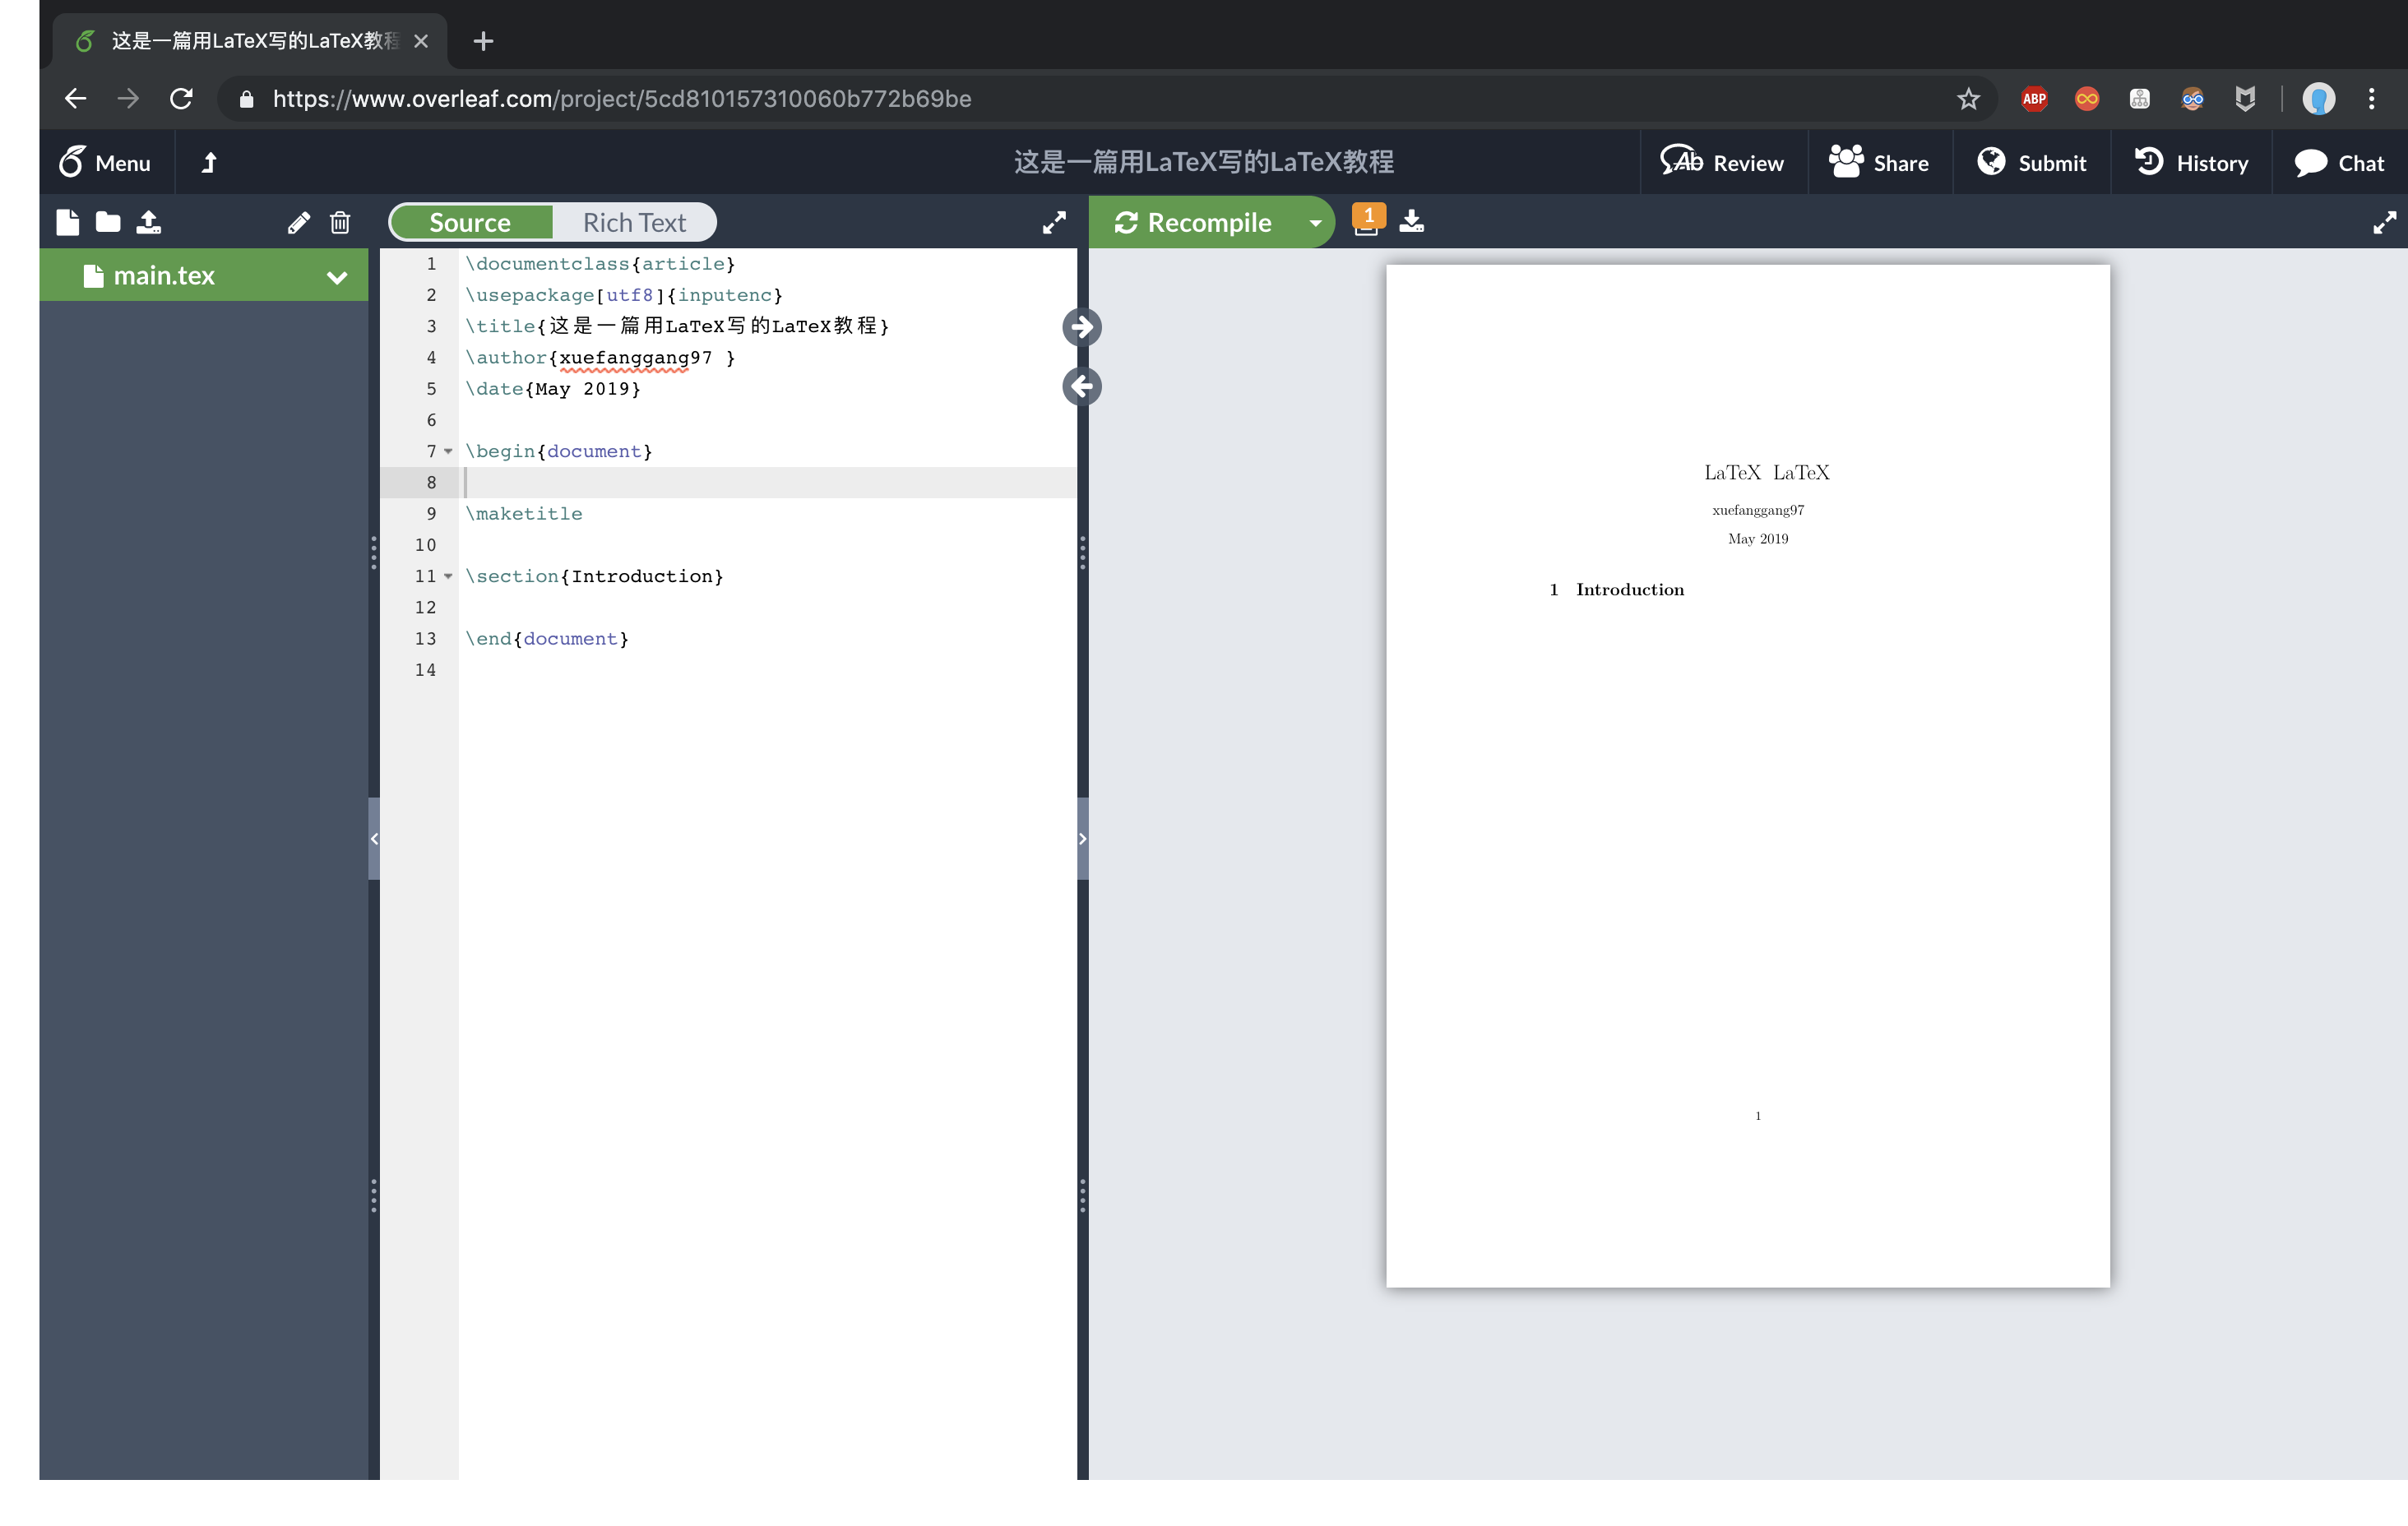
\includegraphics[width=1\textwidth]{init-page.png}
\caption{新项目初始页面}
\label{init-page}
\end{figure}

编辑界面分为三栏,从左往右看,第一栏为工具栏,主要用作对项目的配置和管理,第二栏是编辑界面,主要用来编写代码,第三栏是预览栏,主要是预览作用。可能细心的同学已经发现,我这里新建完项目之后右边预览栏中的标题是没有正确显示的(正常应该显示”这是一片用LateX编写的LaTeX教程“,此处显示为”latex...“),这是因为overleaf默认是不支持中文的,所以我们需要配置一下,让当前项目支持中文,当然如果你是准备写英文就可以不用配置。具体的配置分为2步:\\
1:添加ctex宏包\\
将代码 $\backslash$usepackage\{ctex\}添加到你代码的顶部即可。\\
2:配置使用 xelatex 引擎编译\\
如图\ref{set-xelatex}所示,在左边第一栏中点击”Menu“,然后设置Complier为xelatex。\\
\begin{figure}[H]
\centering
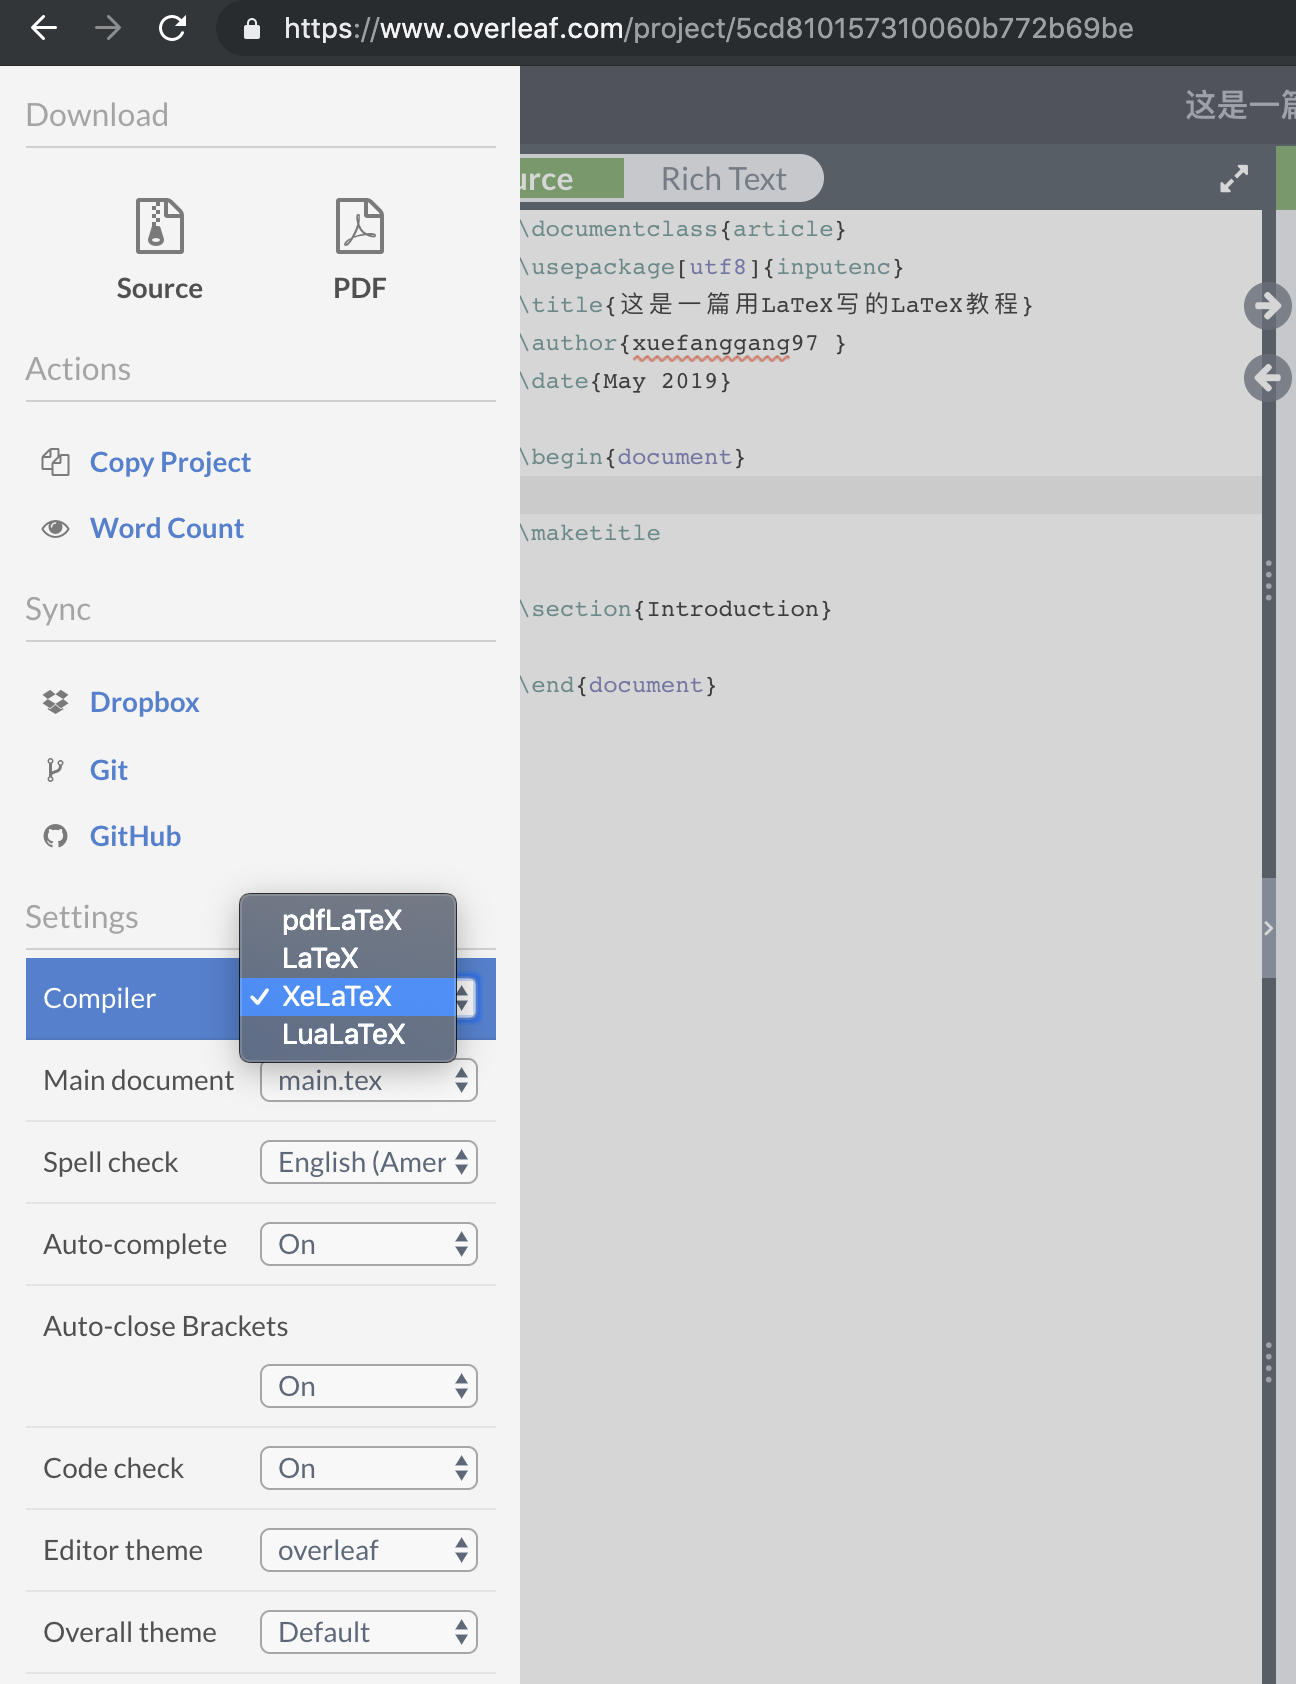
\includegraphics[width=1\textwidth]{设置编译器为xelatex.png}
\caption{设置编译器为xelatex}
\label{set-xelatex}
\end{figure}
完成了以上两步之后,你的当前项目就可以完美支持中文了,你就可以开始你愉快的写作了。\\
接下来我来介绍一下LaTeX常用的一些操作。

\section{LateX基本使用}
\subsection{文本\&排版}
\subsubsection{定版型}
$\backslash$documentclass [参数A] {参数B}
\begin{itemize}
\item[参数A] 

\begin{enumerate}[1]
\item 字体10pt(默认值),11pt,12pt,例子:$\backslash$documentclass[11pt]{article};
\item 纸张大小有几个,最常见的就是a4paper,letterpaper(默认值),例子:$\backslash$documentclass[a4paper]\{article\};
\item 单双面oneside(article,report默认值),twoside(book默认值),例子:$\backslash$documentclass[twoside]\{article\};
\item 组合实现:$\backslash$documentclass[a4paper,twoside,11pt]\{article\}顺序随意;
\end{enumerate}

\item[参数B] 
\begin{enumerate}[1]
    \item 常用:Article(英文科研文章)/report/book;
    \item ctex文档类(支持中文):ctexart/ctexrep/ctexbook;
\end{enumerate}

\end{itemize}

\subsubsection{加标题/日期/作者}

在$\backslash$begin\{document\}之前输入:$\backslash$title{标题}$\backslash$author{作者}$\backslash$date{日期} ,输入空格即为空

在$\backslash$begin\{document\}之前输入:$\backslash$maketitle ,  输入后,前三者才生效        


\subsubsection{修改页边距}
首先需要导入宏包:$\backslash$usepackage\{geometry\}\\
然后使用:$\backslash$gemometry(left=2.54cm,rught=2.54cm,top=3.09cm,bottom=3.09cm),表示A4版上下为 2.54厘米,左右为 3.09厘米

\subsubsection{文本加粗}
$\backslash$textbf\{ 需要加粗的内容\}

\subsubsection{左对齐}
$\backslash$noindent ,表示本行左对齐不缩进

\subsubsection{换行}
$\backslash$newline或者 $\backslash$ $\backslash$

\subsubsection{空格}
单空格$\backslash$quad ,双空格$\backslash$ $\backslash$quad

\subsubsection{居中/左对齐/右对齐}
\begin{itemize}
    \item 部分居中\\
    $\backslash$centering,小范围内(比如表格)居中后面部分内容
    \item 全部居中/左对齐/右对齐\\
    $\backslash$begin{center/flushleft/flushright}\\要居中的内容\\
    $\backslash$end{center/flushleft/flushright };
\end{itemize}

\subsection{公式编辑}
\subsubsection{插入公式}
\begin{itemize}
    \item 行内插入公式:\$公式\$
    \item 行间插入公式(自动为公式编号):\$\$公式\$\$
\end{itemize}
\subsubsection{粗体}
粗体主要是写向量或矩阵的时候会需要加粗,用法:
$\backslash$mathbf\{\}

\subsubsection{上下标}
\begin{itemize}
    \item 上标:\^,比如:a\^2表示$a^2$
    \item 下标:\_,比如:a\_2表示$a_2$
\end{itemize}

\subsubsection{分数}
$\backslash$frac\{分子\}\{分母\}
\subsubsection{累和、累积}
\begin{itemize}
    \item 累和:$\backslash$sum\_\{下标\}\{上标\},比如\$sum\_\{n=1\}\{100\}\$的结果为$\sum_{n=1}{100}$
    \item 累积:$\backslash$prod\_\{下标\}\{上标\},比如\$prod\_\{n=1\}\{100\}\$的结果为$\prod_{n=1}{100}$
    
\end{itemize}

\subsubsection{常用符号表}
常用的符号表如下面几张图所示:
 \begin{figure}[H]
\centering
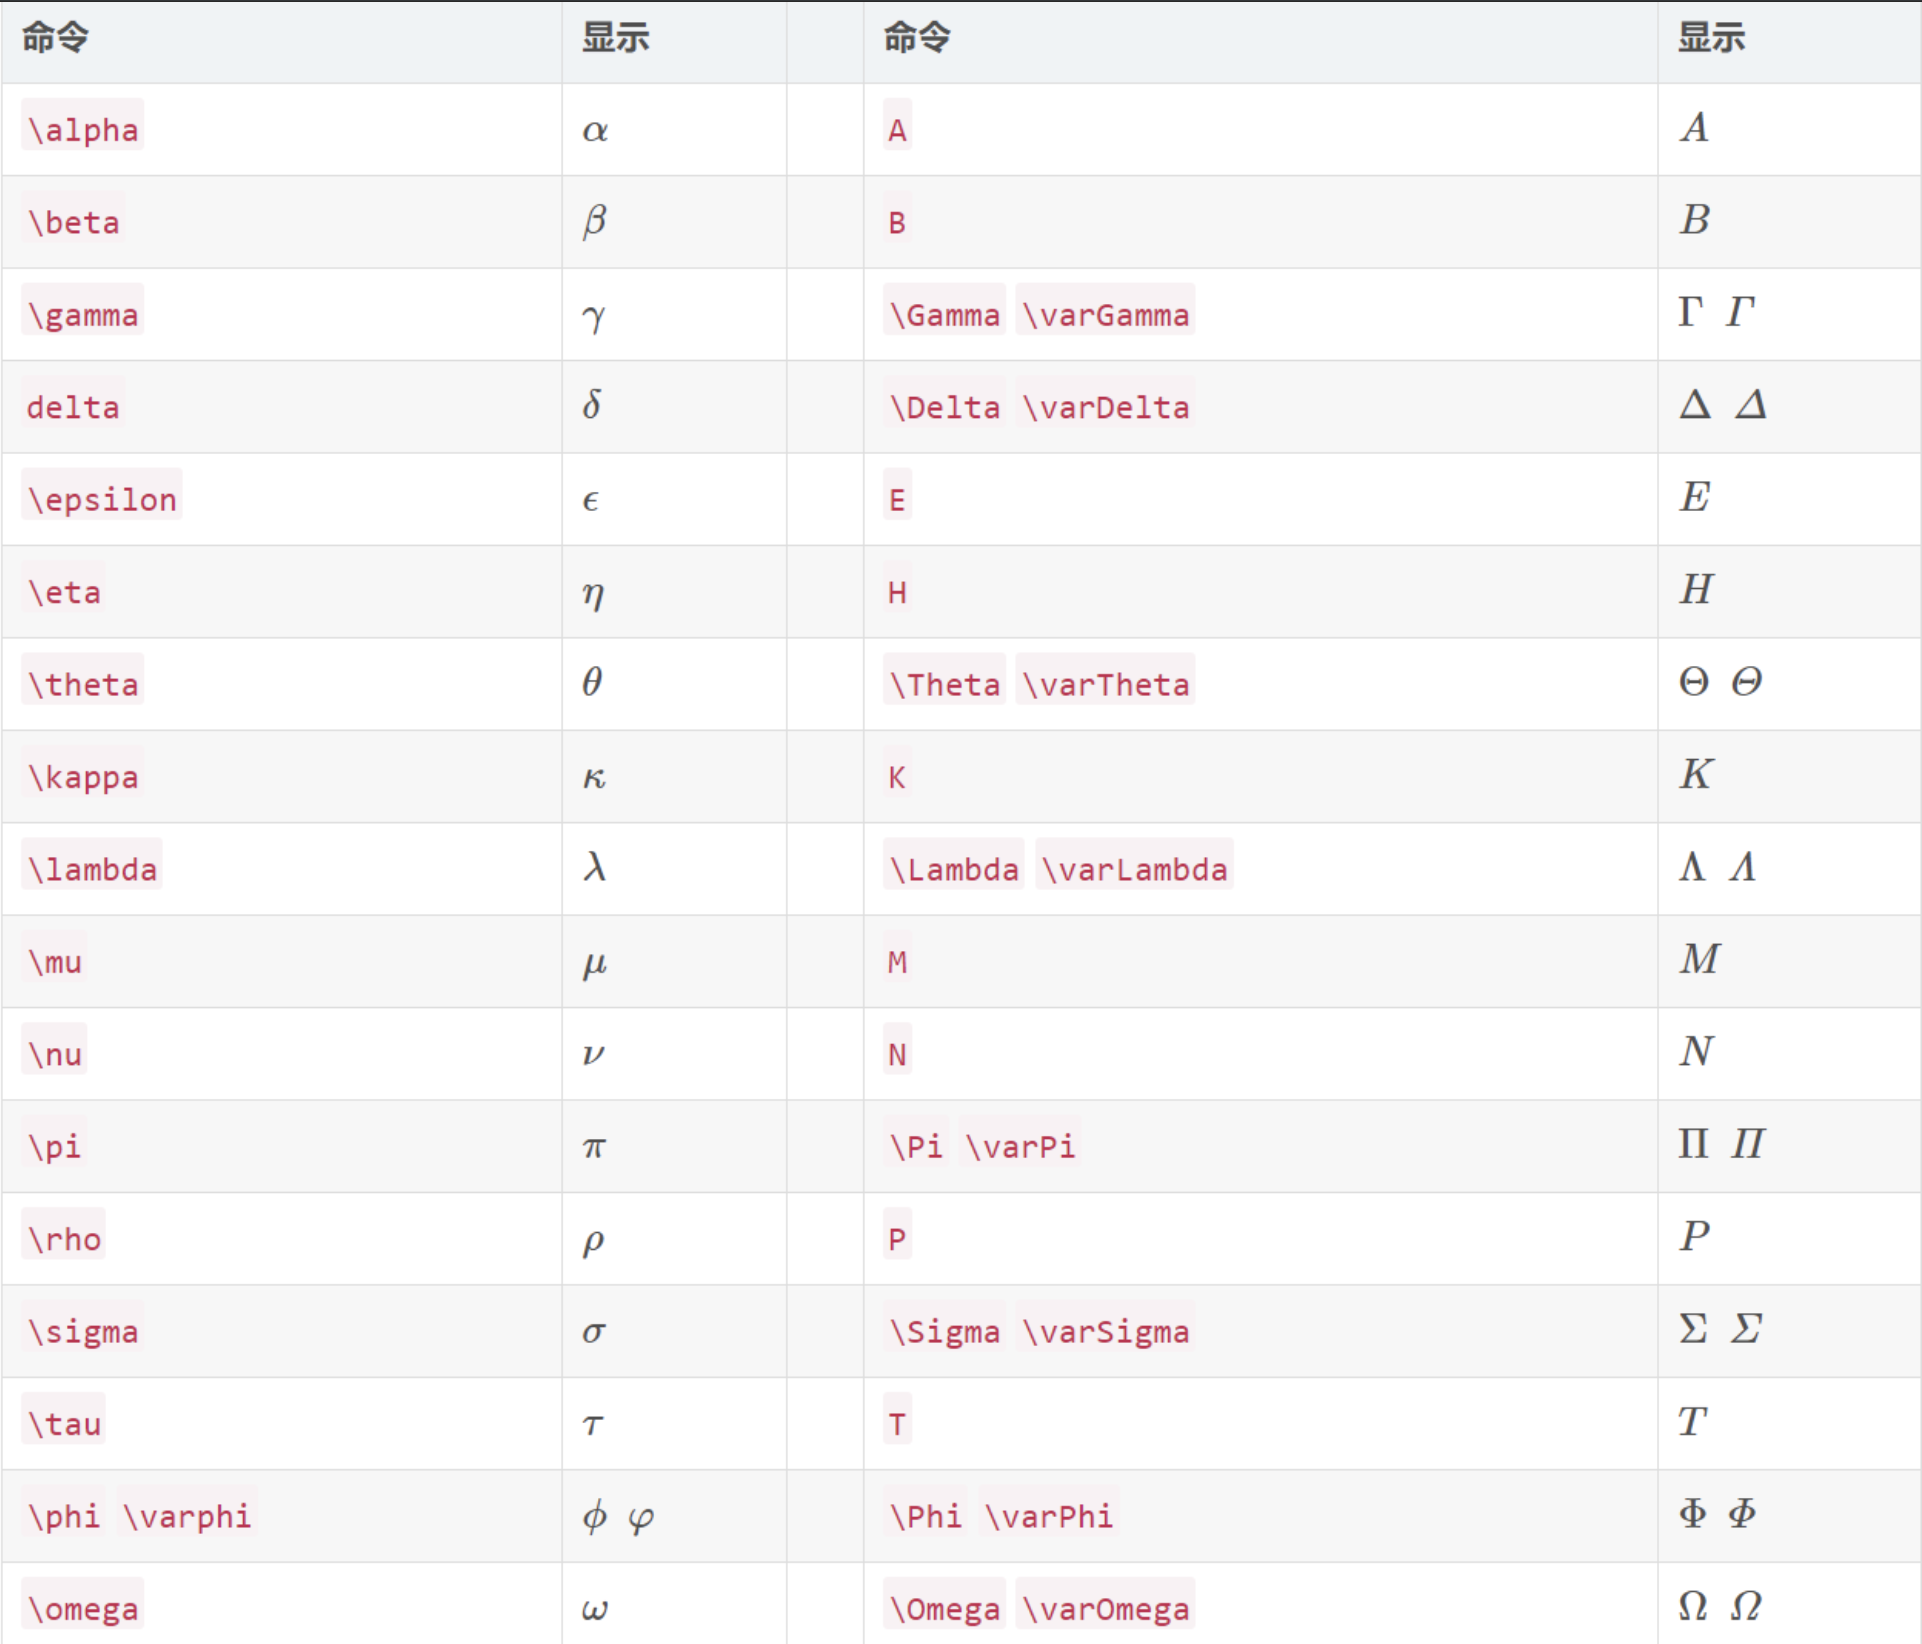
\includegraphics[width=1\textwidth]{希腊字母.png}
\caption{希腊字母}
\label{xila}
\end{figure}


 \begin{figure}[H]
\centering
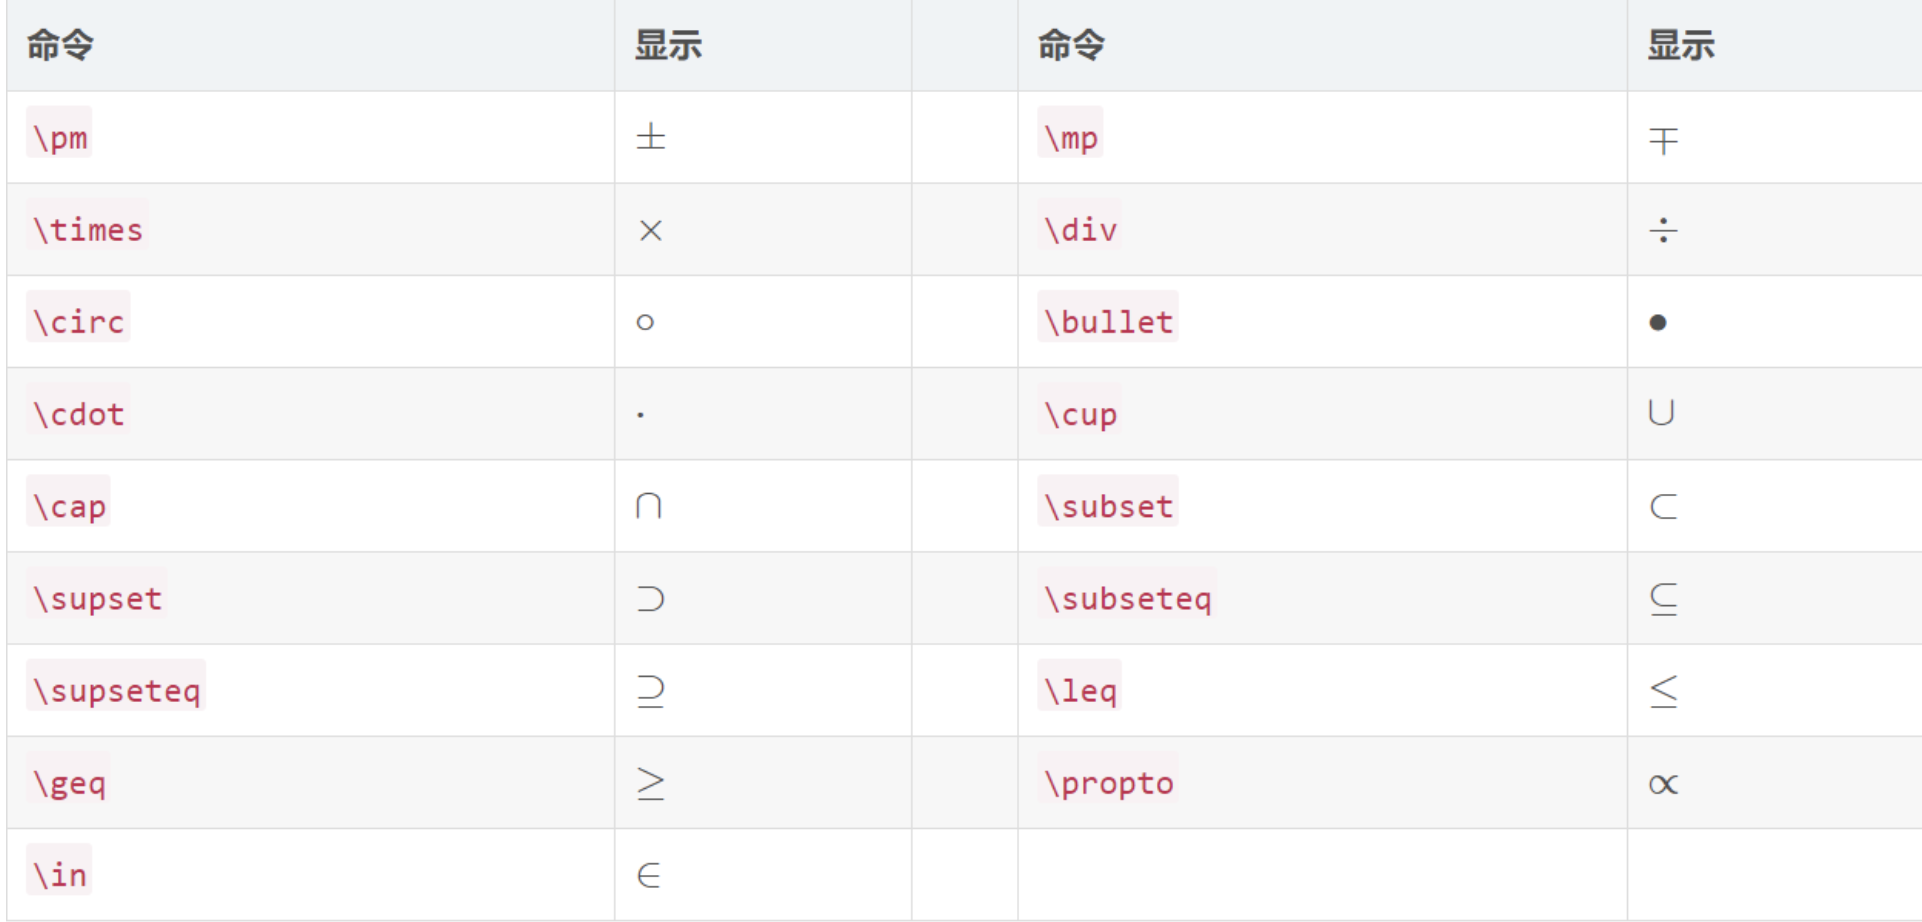
\includegraphics[width=1\textwidth]{基本运算符.png}
\caption{基本运算符}
\label{jibenyunsuanfu}
\end{figure}

 \begin{figure}[H]
\centering
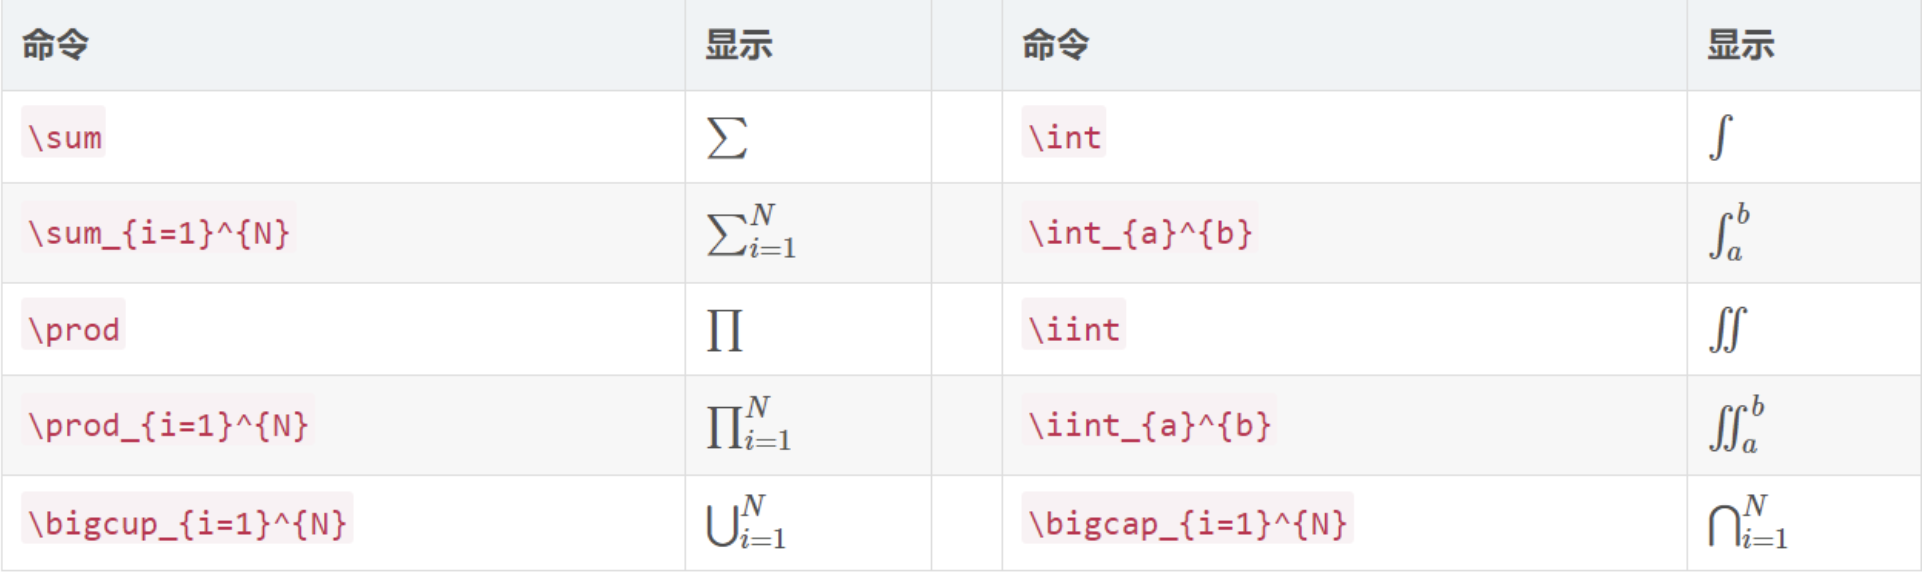
\includegraphics[width=1\textwidth]{积分运算符.png}
\caption{积分运算符}
\label{jifen}
\end{figure}

 \begin{figure}[H]
\centering
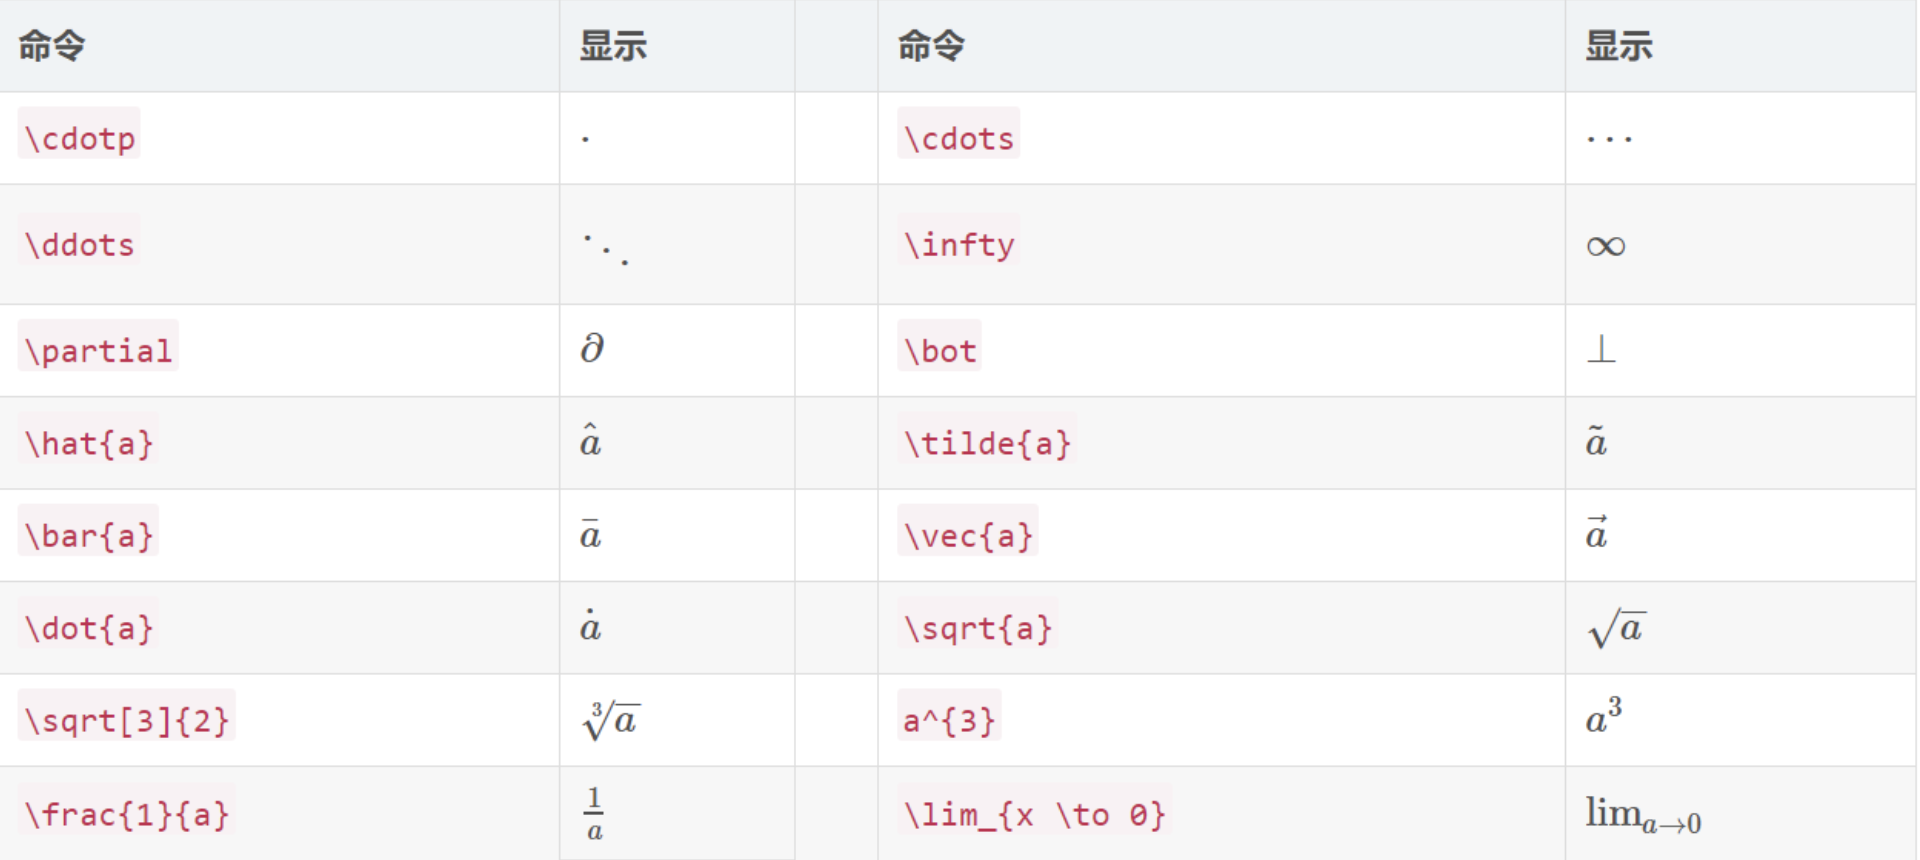
\includegraphics[width=1\textwidth]{其他符号.png}
\caption{其他符号}
\label{qita}
\end{figure}

\subsection{插入图片}
插入图片需要2步:\\
\subsubsection{将本地图片上传到OverLeaf的项目中}

 \begin{figure}[H]
\centering

\includegraphics[width=1\textwidth]{upload-pic.png}
\caption{上传图片示意图-1}
\label{upload-pic}
\end{figure}

如图\ref{upload-pic}所示,点击menu栏的上传图标,然后就可以看到如图\ref{select-pic}所示的选择界面,然后点击那个绿色按钮就可以选择你本地的图片进行上传,当然你也可以直接将本地的图片拖拽到相应的区域上传。

\begin{figure}[H]
\centering
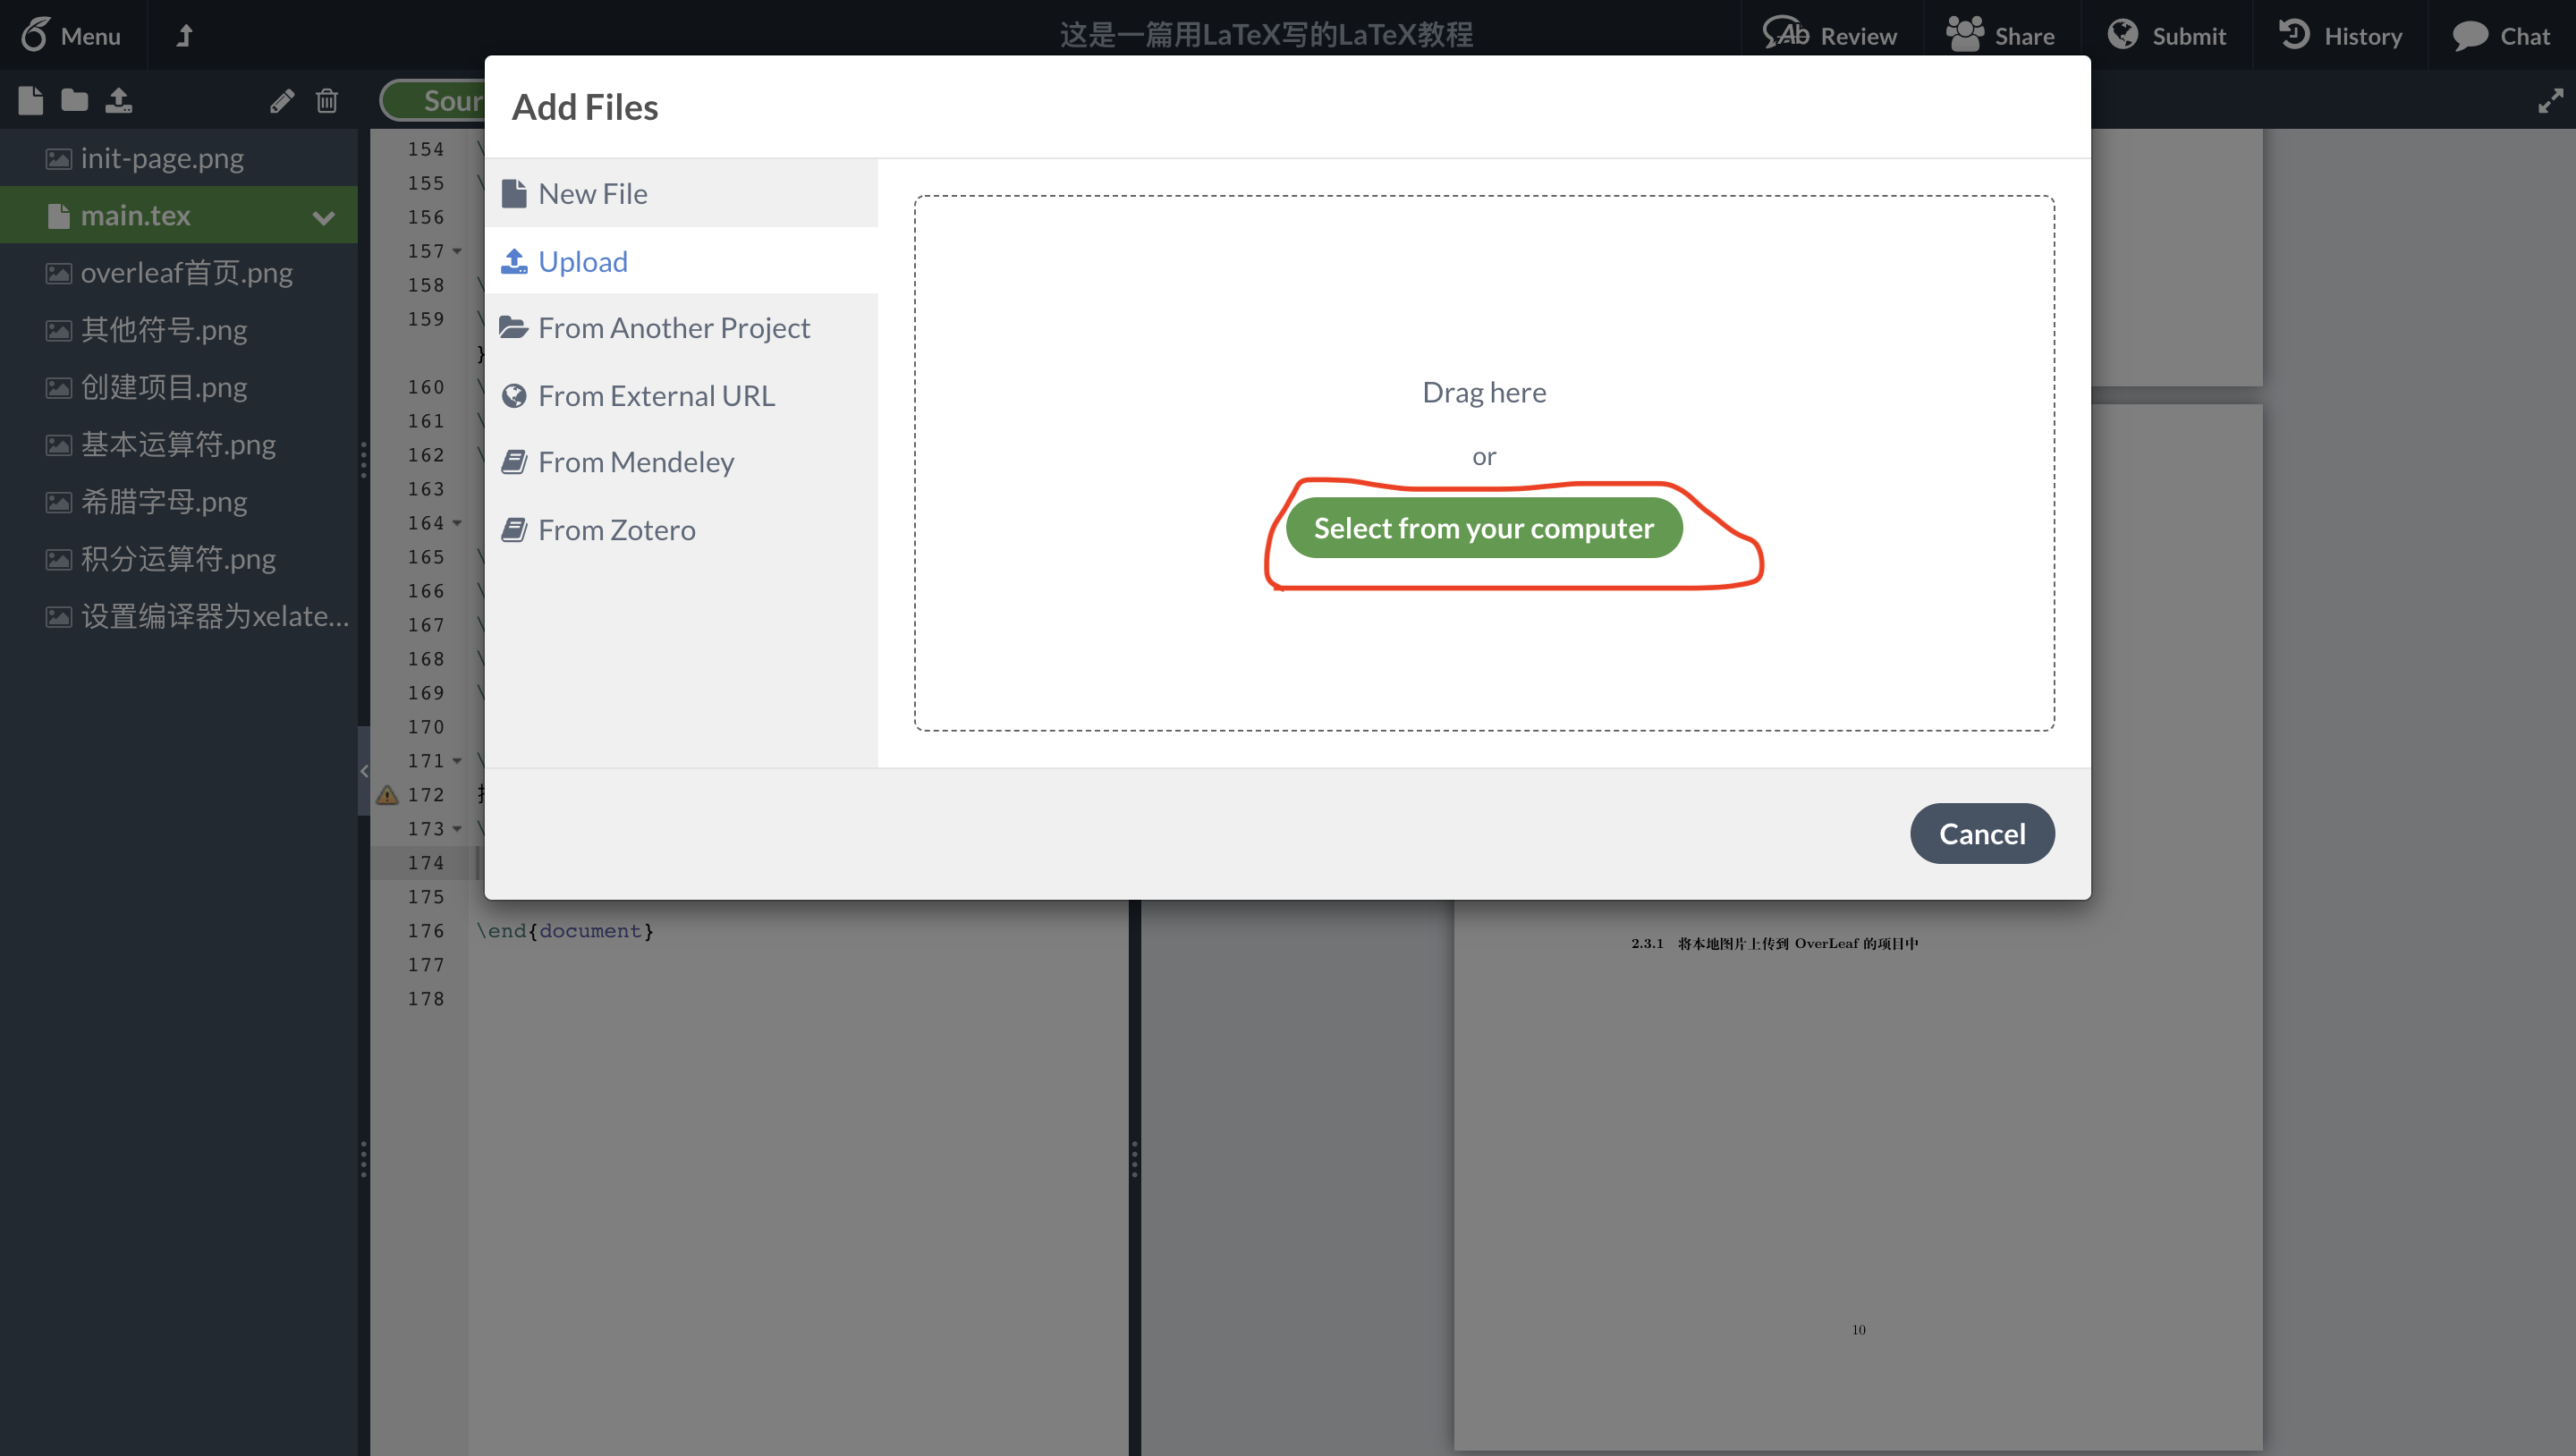
\includegraphics[width=1\textwidth]{select-pic.png}
\caption{上传图片示意图-2}
\label{select-pic}
\end{figure}
\subsubsection{编写代码将图片插入到正文中}
将图片成功上传到OverLeaf的项目中后就可以编写代码在正文中插入相应的图片了,代码的编写规则如下:
\begin{lstlisting}

\usepackage{graphicx} %加入头文件\\
    \begin{figure}[!htpb]/[H] %[htbp]是自动排版;[H]固定位置 
        \centering %图片居中         
        \includegraphics[scale=0.3]/[width=4.5in]{DPBS.png} %设置大小和名称 
        \caption{DPBS}
        \label{1} %图片名称和图片标号 
    \end{figure} %结束 
\end{lstlisting}
其中,{figure}的可选参数[!htbp]: ; 
\begin{itemize}
    \item 『h』当前位置。将图形放置在正文文本中给出该图形环境的地方。如果本页所剩的页面不够,这一参数将不起作用。
\item『t』顶部。将图形放置在页面的顶部。
\item『b』底部。将图形放置在页面的底部。
\item『p』浮动页。将图形放置在一只允许有浮动对象的页面上。
\end{itemize}

如果想让图片出现在你编写代码的对应位置(默认情况下图片是自定根据美观调整位置的)一般使用[htb]这样的组合,只用[h]是没有用的。这样组合的意思就是latex会尽量满足排在前面的浮动格式,就是h-t-b这个顺序,让排版的效果尽量好。\\
!h 只是试图放在当前位置。如果页面剩下的部分放不下,还是会跑到下一页的。一般页言,用 [!h] 选项经常会出现不能正确放置的问题,所以常用 [ht]、[htbp] 等。

如果你一定需要把图片放在当前位置,不容改变,可以用float宏包的[H]选项。不过如果这样做,出现放不下的问题时需要手工调整。使用格式如下:
$\backslash$usepackage{float}

\subsection{插入表格}



\subsubsection{粗线(表格的第一根线和最后一根线比表格中的横线更粗一些)}

导入宏包:$\backslash$usepackage\{booktabs\} 

$\backslash$toprule ,第一根线

    $\backslash$midrule  ,中间的线
    
    $\backslash$bottomrule ,最后一根线

\subsubsection{调整位置}
$\backslash$begin\{table\}[!htbp]

$\backslash$end\{table\}
其中,\{table\}有若干可选参数[!htbp]
\begin{itemize}
    \item h代表here,将表格排在当前文字位置 ;
    \item t表示将表格放在下一页的 top (页首) ;
    \item p表示p-page-of-its-own;
    \item b表示将表格放在当前页的 bottom (底部);
    \item !表示忽略美观因素,尽可能按照参数指定的方式来处理表格浮动位置;
\end{itemize}

\subsubsection{居中}
长度不长时:$\backslash$centering

长度过长时:$\backslash$centerline\{\} ,把tabular的所有内容放进去                      

\subsubsection{制表}



$\backslash$begin\{tabular\}\{|l |c | r |\},“|”表示竖线,“l/c/r”表示格内文字居左/中/右显示

A \& B \& C$\backslash$ $\backslash$               

E \& F \& G$\backslash$ $\backslash$   

$\backslash$end\{tabular\}

“\&”分隔不同列内的内容,“$\backslash$ $\backslash$”表示换行

\subsubsection{列的合并(合并一行多列)}
我们使用$\backslash$multicolumn\{项数\}\{新列格式\}\{内容\} 命令将一行中的几个不同的表格合并为一项。\\
比如原本有一个表格是这样的:
\begin{lstlisting}
        \begin{tabular}{|c|c|c|}
        \hline
        
        成绩1 &   成绩2  & 总计\\ 
        \hline
        
        语文  &   数学 & \\   
        \hline
        
        87    & 100 &187  \\
        \hline
        
        \end{tabular}
\end{lstlisting}
绘制出来效果如表\ref{table1}所示.
\begin{table}[H]
    \centering
    \begin{tabular}{|c|c|c|}
        \hline
        
        成绩1 &   成绩2  & 总计\\ 
        \hline
        
        语文  &   数学  & \quad \\   
        \hline
        
        87    & 100 &187  \\
        \hline
        
        \end{tabular}
    \caption{合并列之前的表格}
    \label{table1}
\end{table}

现在我们需要将\ref{table1}的第1行的两列(成绩1、成绩2)合并成为1列(成绩),我们应该使用$\backslash$multicolumn\{合并的列数\}\{新列格式\}\{合并后行的内容\} 命令:
\begin{lstlisting}
       \begin{tabular}{|c|c|c|}
            \hline
        
            \multicolumn{2}{|c|}
            {成绩}&总计  \\ 
            %合并本行的2项,新列的格式是,2项合并后的本列的格式是|c|,合并后本格的内容是{成绩}&总计
            
            \hline
        
            语文  &   数学 & \quad \\   
            \hline
            
            87    & 100 & 187 \\
            \hline
        
        \end{tabular}
\end{lstlisting}

绘制出来的表格如表\ref{table2}所示

\begin{table}[H]
    \centering
        \begin{tabular}{|c|c|c|}
            \hline
        
            \multicolumn{2}{|c|}
            {成绩}&总计  \\ %,合并本行的2项,新列的格式是
            \hline
        
            语文  &   数学 & \quad \\   
            \hline
            
            87    & 100 & 187 \\
            \hline
        
        \end{tabular}
    \caption{合并列以后的表格}
    \label{table2}
\end{table}

在这里需要注意的一个地方就是当我们使用了$\backslash$multicolumn\{合并的列数\}的时候这个时候我们在表头定义的格式就会完全对我们重新合并的单元格失去作用,所以我们自己必须重新定义新的格式。也就是我们例子中的这个样子$\backslash$multicolumn\{2\}\{|c|\}

\subsubsection{行的合并(合并一列多行)}
合并多行1列单元格可以用multirow包中的$\backslash$multirow\{合并的行数\}\{宽度\}\{合并后列中的内容\}来实现,注意和$\backslash$multicolumn命令的2点不同:
\begin{itemize}
    \item $\backslash$multicolumn不需要导入任何宏包可以直接使用,$\backslash$multirow必须使用$\backslash$usepackage\{multirow\}导入multirow这个宏包
    \item $\backslash$multirow\{合并的行数\}\{宽度\}\{合并后列中的内容\}中的第2个参数是\{宽度\},与$\backslash$multicolumn第2个参数不同。如果不确定\{宽度\}需要填什么,就将其替换为*,如下面代码块中所示
\end{itemize}

例如如下表格:
\begin{lstlisting}
        \begin{tabular}{|c|c|c|}
        \hline
        
        成绩1 &   语文  & 87\\ 
        \hline
        
        成绩2  &   数学  & 100 \\   
        \hline
        
        总计    & \quad &187  \\
        \hline
        
        \end{tabular}
\end{lstlisting}
其绘制出来如表\ref{table3}:
\begin{table}[H]
    \centering
    \begin{tabular}{|c|c|c|}
        \hline
        
        成绩1 &   语文  & 87\\ 
        \hline
        
        成绩2  &   数学  & 100 \\   
        \hline
        
        总计    & \quad &187  \\
        \hline
        
        \end{tabular}
    \caption{合并行之前的表格}
    \label{table3}
\end{table}
现在我们想合并第1列的前2行,应该使用如下代码:
\begin{lstlisting}
        \begin{tabular}{|c|c|c|}
        \hline
        \multirow{2}*{成绩}
        
        ~ & 语文  & 87\\ 
        \cline{2-3}

         ~ & 数学  & 100 \\  
         \hline
        
        总计    & \quad &187  \\
        \hline
        
        \end{tabular}
\end{lstlisting}
绘制完成之后的效果如表\ref{table4}所示:
\begin{table}[H]
    \centering
    \begin{tabular}{|c|c|c|}
        \hline
        \multirow{2}*{成绩}
        
        
        & 语文  & 87\\ 
        \cline{2-3}

        
         & 数学  & 100 \\  
         
         \hline
      
        
        总计    & \quad &187  \\
        \hline
        
        \end{tabular}
    \caption{合并行之后的表格}
    \label{table4}
\end{table}
这里需要注意2点:

\begin{itemize}
    \item 第3行的$\backslash$multirow的第2个参数使用了\*,注意不是\{\*\}哦
    
    \item 第5行的“\~\& 语文  \& 87$\backslash$ $\backslash$”和第8行的“\~\& 数学  
    \& 100 $\backslash$ $\backslash$“中都有个\~其实这个\~不是必须要的,但是~后面紧跟的那个\&是必须的,它起到一个占位作用,不然编译器怎么知道你要合并的是哪个位置的2行(是1-2行还是2-3行),我这里为了更加显眼写了个\~,大家在实际使用的时候可以省略\~,但是\~后面的那个\&是绝对不能省的
    
    \item 第6行使用了$\backslash$cline\{2-3\}来画这一行的直线,没有使用$\backslash$hline,因为$\backslash$hline绘制的是从表格开始到表格结束的一行直线,很明显我们这里只需要在第2列到第3列的当前位置绘制一条横线即可,所以使用$\backslash$cline\{2-3\}

\end{itemize}


\subsubsection{合并行的同时合并列}
其实只要学会了合并行和合并列,这里只要将二者同时使用即可,这里给出一个示例:
    
\begin{lstlisting}
  
         \begin{tabular}{|c|c|c|}
        \hline
        \multicolumn{2}{|c|}
        {姓名}&小草莓\\
       
        \hline
        
        \multirow{2}*{成绩}
        & 语文  & 87\\ 
        \cline{2-3}

        
         & 数学  & 100 \\  
         
         \hline
      
        
        总计    & \quad &187  \\
        \hline
        
        \end{tabular}
\end{lstlisting}
绘制完成后如表\ref{table5}所示:
\begin{table}[H]
    \centering
    \begin{tabular}{|c|c|c|}
        \hline
        \multicolumn{2}{|c|}
        {姓名}&小草莓\\
       
        \hline
        
        \multirow{2}*{成绩}
        & 语文  & 87\\ 
        \cline{2-3}

        
         & 数学  & 100 \\  
         
         \hline
      
        
        总计    & \quad &187  \\
        \hline
        
        \end{tabular}
    \caption{合并行和列}
    \label{table5}
\end{table}

\subsubsection{标签和名称}
$\backslash$label\{label\}$\backslash$caption\{name\} 

\subsubsection{普通线}
$\backslash$hline或$\backslash$cline\{2-5\}            ,两者都是用来画水平的表格线,但是$\backslash$cline可以用来指定画线的起始和终止位置

$\backslash$subsubsection\{行高\}
$\backslash$renewcommand$\backslash$arraystretch\{2\} ,表格行高设置为默认的2倍



\subsection{参考文献的书写}

$\backslash$begin\{thebibliography\}\{\}

    $\backslash$bibitem\{ref label\}

    内容
    
\{$\backslash$em要斜体的内容\} 
\{$\backslash$bf要加粗的内容\}

$\backslash$end\{thebibliography\}

\begin{thebibliography}{}
\bibitem{ref 1.1} 
微信公众号"IT工匠"
\end{thebibliography} 
\end{document}

